% Importado desde: 2026-03-28_Consistencia_Global_Brillouin_Nielsen_QW_Dirac.tex
\chapter{Derivacion Pedagogica: --- consistencia global del protoespacio discreto: --- Brillouin, cuasienergia y Nielsen--Ninomiya}
\label{ch:consistencia-global-brillouin}

\section{Objetivo}
En el capitulo anterior dimos un paso importante: dejamos de pensar solo en el sector infrarrojo y preguntamos que objeto discreto global sostiene realmente a la dinamica efectiva de Dirac.

Ahora toca atacar la prueba dura de consistencia global. Eso significa estudiar:
\begin{enumerate}[label=\arabic*.]
    \item la zona de Brillouin completa;
    \item la cuasienergia exacta del paso unitario;
    \item los puntos especiales fuera del parche infrarrojo;
    \item y como entra Nielsen--Ninomiya en esta construccion discreta de tipo \textit{quantum walk}.
\end{enumerate}

La pregunta central del capitulo es:
\begin{displayquote}
\textbf{que exige la estructura global del toro de Brillouin al intento de obtener Dirac \(3+1\) desde una microdinamica discreta?}
\end{displayquote}

\section{El objeto exacto que estamos estudiando}
Tomamos como bloque elemental la caminata Weyl
\begin{equation}
U_W(\vk)=
\ee^{-\,\ii a k_z \sigma_z}
\ee^{-\,\ii a k_y \sigma_y}
\ee^{-\,\ii a k_x \sigma_x},
\label{c32:eq:UW}
\end{equation}
con
\begin{equation}
\vk \in T^3
=
\mathbb{R}^3/\frac{2\pi}{a}\mathbb{Z}^3.
\end{equation}

El objeto global no vive entonces sobre \(\mathbb{R}^3\), sino sobre el toro de Brillouin \(T^3\), y la energia se reemplaza por cuasienergia.

\subsection{Forma canonica}
Como \(U_W(\vk)\in SU(2)\), puede escribirse como
\begin{equation}
U_W(\vk)=
\cos\!\bigl(\omega(\vk)\Delta t\bigr)\,\bbI
-\ii \sin\!\bigl(\omega(\vk)\Delta t\bigr)\,\hat{\bm{n}}(\vk)\cdot\vsigma.
\label{c32:eq:canon}
\end{equation}

La traza fija la cuasienergia:
\begin{equation}
\cos\!\bigl(\omega(\vk)\Delta t\bigr)
=
\cos(ak_x)\cos(ak_y)\cos(ak_z)
+ \sin(ak_x)\sin(ak_y)\sin(ak_z).
\label{c32:eq:omega}
\end{equation}

\section{Primera leccion global: la cuasienergia es circular}
En tiempo discreto, la cuasienergia no vive en la recta real, sino en un circulo:
\begin{equation}
\omega \sim \omega + \frac{2\pi}{\Delta t}.
\end{equation}

Eso significa que hay dos lugares naturalmente especiales:
\begin{enumerate}[label=\arabic*.]
    \item \(\omega = 0\);
    \item \(\omega = \pi/\Delta t\).
\end{enumerate}

Este punto ya diferencia fuertemente la historia discreta de la historia hamiltoniana continua.

\begin{displayquote}
\textbf{en un sistema unitario por pasos, los nodos relevantes no tienen por que vivir todos en \(\omega=0\); tambien pueden vivir en la zona \(\omega=\pi/\Delta t\).}
\end{displayquote}

\section{Los puntos especiales de la zona de Brillouin}
Tomemos los ocho vertices del cubo de Brillouin:
\begin{equation}
\vk^{(n_x n_y n_z)}=
\left(
\frac{n_x\pi}{a},
\frac{n_y\pi}{a},
\frac{n_z\pi}{a}
\right),
\qquad
n_i\in\{0,1\}.
\label{c32:eq:corners}
\end{equation}

En esos puntos:
\begin{equation}
\sin(n_i\pi)=0,
\qquad
\cos(n_i\pi)=(-1)^{n_i}.
\end{equation}

Entonces \eqref{c32:eq:omega} se reduce a
\begin{equation}
\cos\!\bigl(\omega\Delta t\bigr)
=
(-1)^{n_x+n_y+n_z}.
\label{c32:eq:corneromega}
\end{equation}

\subsection{Clasificacion de la familia de esquinas}
Luego, restringidos a esta familia de esquinas:
\begin{enumerate}[label=\arabic*.]
    \item si \(n_x+n_y+n_z\) es par, entonces \(\cos(\omega\Delta t)=+1\), o sea \(\omega=0\) modulo \(2\pi/\Delta t\);
    \item si \(n_x+n_y+n_z\) es impar, entonces \(\cos(\omega\Delta t)=-1\), o sea \(\omega=\pi/\Delta t\) modulo \(2\pi/\Delta t\).
\end{enumerate}

Por tanto, dentro de esta familia:
\begin{equation}
\boxed{
4\ \text{esquinas en } \omega=0,
\qquad
4\ \text{esquinas en } \omega=\pi/\Delta t.
}
\label{c32:eq:fourfour}
\end{equation}

\begin{displayquote}
\textbf{Advertencia importante.} Esta cuenta clasifica solo los ocho vertices del dominio fundamental. No demuestra todavia que esos sean \emph{todos} los puntos especiales del espectro global.
\end{displayquote}

\begin{figure}[h!]
\centering
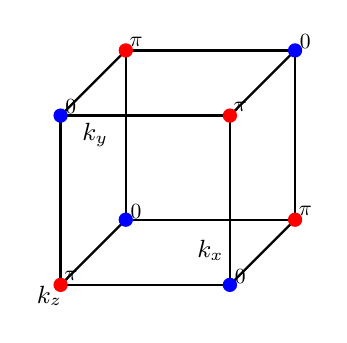
\begin{tikzpicture}[scale=2.15]
\draw[thick] (0,0,0) -- (1,0,0);
\draw[thick] (0,0,0) -- (0,1,0);
\draw[thick] (0,0,0) -- (0,0,1);
\draw[thick] (1,0,0) -- (1,1,0);
\draw[thick] (1,0,0) -- (1,0,1);
\draw[thick] (0,1,0) -- (1,1,0);
\draw[thick] (0,1,0) -- (0,1,1);
\draw[thick] (0,0,1) -- (1,0,1);
\draw[thick] (0,0,1) -- (0,1,1);
\draw[thick] (1,1,0) -- (1,1,1);
\draw[thick] (1,0,1) -- (1,1,1);
\draw[thick] (0,1,1) -- (1,1,1);

\foreach \x/\y/\z/\col/\lab in {
0/0/0/blue/{\(0\)},
1/0/0/red/{\(\pi\)},
0/1/0/red/{\(\pi\)},
0/0/1/red/{\(\pi\)},
1/1/0/blue/{\(0\)},
1/0/1/blue/{\(0\)},
0/1/1/blue/{\(0\)},
1/1/1/red/{\(\pi\)}}
{
  \fill[\col] (\x,\y,\z) circle (1.2pt);
  \node[scale=0.78] at (\x+0.08,\y+0.07,\z+0.05) {\lab};
}
\node at (0.5,-0.18,0) {\small \(k_x\)};
\node at (-0.18,0.5,0) {\small \(k_y\)};
\node at (0,0,1.17) {\small \(k_z\)};
\end{tikzpicture}
\caption{Los ocho vertices del dominio fundamental de Brillouin se reparten en dos familias: cuatro en cuasienergia \(0\) y cuatro en cuasienergia \(\pi/\Delta t\).}
\end{figure}

\section{Linealizacion alrededor de cada punto}
Sea
\begin{equation}
\vk = \vk^{(n_x n_y n_z)}+\vq,
\qquad
\abs{\vq}\ll \frac{\pi}{a}.
\end{equation}

Entonces:
\begin{equation}
\sin(n_i\pi + q_i a)\simeq (-1)^{n_i}q_i a,
\qquad
\cos(n_i\pi + q_i a)\simeq (-1)^{n_i}.
\end{equation}

\subsection{Sector de \(\omega=0\)}
Cuando la paridad es par, el paso se expande como
\begin{equation}
U_W \simeq
\bbI
-\ii a\left(
(-1)^{n_x}\sigma_x q_x
+(-1)^{n_y}\sigma_y q_y
+(-1)^{n_z}\sigma_z q_z
\right).
\end{equation}

Luego el Hamiltoniano efectivo local es
\begin{equation}
H^{(0)}_{(n)}(\vq)
=
v\left(
(-1)^{n_x}\sigma_x q_x
+(-1)^{n_y}\sigma_y q_y
+(-1)^{n_z}\sigma_z q_z
\right).
\label{c32:eq:H0}
\end{equation}

\subsection{Sector de \(\omega=\pi/\Delta t\)}
Cuando la paridad es impar, el paso se expande como
\begin{equation}
U_W \simeq
-\bbI
+\ii a\left(
(-1)^{n_x}\sigma_x q_x
+(-1)^{n_y}\sigma_y q_y
+(-1)^{n_z}\sigma_z q_z
\right).
\end{equation}

Factorizando la fase global \(e^{-i\pi}=-1\):
\begin{equation}
U_W \simeq
e^{-i\pi}
\left[
\bbI
-\ii \Delta t\,H^{(\pi)}_{(n)}(\vq)
\right],
\end{equation}
con
\begin{equation}
H^{(\pi)}_{(n)}(\vq)
=
-\,v\left(
(-1)^{n_x}\sigma_x q_x
+(-1)^{n_y}\sigma_y q_y
+(-1)^{n_z}\sigma_z q_z
\right).
\label{c32:eq:Hpi}
\end{equation}

\subsection{Leccion}
Ya dentro de la familia de esquinas, el modelo no tiene un solo cono. Tiene varios conos efectivos repartidos entre dos gaps de cuasienergia distintos: \(0\) y \(\pi\).

\section{Quiralidad y balance en la familia de esquinas}
La matriz de velocidades local es
\begin{equation}
V^{(n)}=
v\,\mathrm{diag}\!\left(
(-1)^{n_x},
(-1)^{n_y},
(-1)^{n_z}
\right)
\end{equation}
en el sector \(0\), y cambia de signo global en el sector \(\pi\).

\subsection{Carga quiral}
La quiralidad local queda determinada por
\begin{equation}
\chi_n = \mathrm{sign}\det V^{(n)}.
\end{equation}

En ambos casos, el patron esencial viene dado por
\begin{equation}
\chi_n = (-1)^{n_x+n_y+n_z}.
\label{c32:eq:chi}
\end{equation}

\subsection{Consecuencia parcial}
Dentro de la familia de esquinas hay cuatro puntos con signo \(+1\) y cuatro con signo \(-1\). Luego, para ese subconjunto:
\begin{equation}
\sum_n \chi_n = 0.
\label{c32:eq:sumzero}
\end{equation}

Esto ya muestra un balance no trivial y va en la direccion esperada por Nielsen--Ninomiya, pero no constituye por si solo una demostracion global completa sobre todo el toro de Brillouin.

\begin{displayquote}
\textbf{no podemos aislar ingenuamente una unica quiralidad ni siquiera dentro de la familia mas simple de esquinas; el balance global completo debe seguir cerrandose.}
\end{displayquote}

\section{Que cambia respecto al caso hamiltoniano ingenuo}
En el modelo hamiltoniano ingenuo, los ocho nodos aparecian todos en energia cero. En la version discreta por pasos ocurre algo mas sutil:
\begin{enumerate}[label=\arabic*.]
    \item dentro de la familia de esquinas, cuatro puntos viven en el gap de cuasienergia \(0\);
    \item y cuatro viven en el gap de cuasienergia \(\pi/\Delta t\).
\end{enumerate}

Eso no destruye la obstruccion global; muestra al menos una primera reorganizacion compatible con ella.

\subsection{Moral}
La consistencia global en un sistema de tiempo discreto debe leerse sobre:
\begin{enumerate}[label=\arabic*.]
    \item el toro de Brillouin \(T^3\);
    \item y el circulo de cuasienergia \(S^1\).
\end{enumerate}

Por eso el objeto exacto es mas rico que el problema estatico de un Hamiltoniano en red.

\section{Insercion del bloque Dirac de cuatro componentes}
Ahora volvemos a la construccion ampliada:
\begin{equation}
U_D = M\,U_0,
\qquad
M=\ee^{-\,\ii \Delta t\,m\,\tau_x\otimes\bbI_2}.
\label{c32:eq:UD}
\end{equation}

Aqui \(U_0\) contiene dos bloques Weyl opuestos.

\subsection{Que hace la masa}
La masa mezcla quiralidades localmente y abre un gap efectivo en el parche infrarrojo que seleccionamos. Pero no destruye el hecho de que el objeto global viva sobre un toro de Brillouin compacto y una cuasienergia periodica.

\subsection{Consecuencia}
Aunque un sector infrarrojo quede muy bien descrito por Dirac \(3+1\), el objeto discreto completo sigue cargando:
\begin{enumerate}[label=\arabic*.]
    \item periodicidad recíproca;
    \item otros puntos especiales;
    \item sectores quirales adicionales;
    \item y una estructura global que no coincide con una teoria relativista unica en todo el espacio de momentos.
\end{enumerate}

\section{Que simetrias exactas sobreviven globalmente}
Ahora podemos responder mejor la pregunta por las simetrias del protoespacio discreto ampliado.

\subsection{Simetrias exactas}
Las mas robustas son:
\begin{enumerate}[label=\arabic*.]
    \item traslaciones discretas de la red;
    \item periodicidad del toro de Brillouin;
    \item discrecion temporal por pasos;
    \item la estructura interna local de cuatro componentes;
    \item y las simetrias puntuales que ademas respeten el orden del paso unitario.
\end{enumerate}

\subsection{Simetrias no exactas}
No son exactas globalmente:
\begin{enumerate}[label=\arabic*.]
    \item la isotropia continua \(SO(3)\);
    \item la simetria de Lorentz completa;
    \item ni una unica estructura Dirac global extendida a todo \(T^3\).
\end{enumerate}

\subsection{Leccion}
El protoespacio discreto no se define por sus simetrias continuas exactas, sino por un paquete mas austero:
\begin{equation}
\text{red discreta}
\;+\;
\text{fibra interna}
\;+\;
\text{paso local}
\;+\;
\text{consistencia topologica global}.
\end{equation}

\section{Que conclusion debemos sacar}
Ahora ya podemos responder con bastante claridad a la intuicion que venias empujando.

\subsection{Respuesta}
Si el sector Dirac es solo infrarrojo, entonces el protoespacio discreto no puede identificarse con el continuo relativista. Debe identificarse con el objeto global que lo sostiene:
\begin{equation}
(\Lambda,\mathbb{C}^4,U_D,T^3,S^1_{\text{cuasienergia}}).
\label{c32:eq:globalobject}
\end{equation}

\subsection{Interpretacion}
Ese objeto no es \enquote{espacio-tiempo} en el sentido usual, pero si puede verse como una preestructura discreta con:
\begin{enumerate}[label=\arabic*.]
    \item localidad;
    \item microcausalidad por pasos;
    \item fibra espinorial local;
    \item y restricciones topologicas globales.
\end{enumerate}

\begin{figure}[h!]
\centering
\begin{tikzpicture}[
    box/.style={draw, rounded corners, thick, align=center, minimum width=3.8cm, minimum height=1.0cm},
    arr/.style={-{Latex[length=3mm]}, thick}
]
\node[box, fill=blue!7] (a) at (0,0) {red \(\Lambda\)\\+ fibra \(\mathbb{C}^4\)};
\node[box, fill=green!7] (b) at (4.7,0) {toro de Brillouin\\+ cuasienergia};
\node[box, fill=yellow!12] (c) at (9.4,0) {balance global\\de quiralidades};
\node[box, fill=red!7] (d) at (14.1,0) {sector Dirac\\solo infrarrojo};
\draw[arr] (a) -- (b);
\draw[arr] (b) -- (c);
\draw[arr] (c) -- (d);
\end{tikzpicture}
\caption{La consistencia global obliga a leer Dirac como sector efectivo de un objeto discreto mas rico.}
\end{figure}

\section{Mapa del siguiente paso}
Si seguimos con rigor, el siguiente paso ya no es volver a derivar Dirac. Es mas bien:
\begin{displayquote}
\textbf{clasificar que clases de pasos unitarios locales permiten minimizar, controlar o reinterpretar la estructura global de dobladores, y bajo que condiciones puede hablarse con propiedad de una proto-geometria discreta estable.}
\end{displayquote}

Eso abre dos rutas naturales:
\begin{enumerate}[label=\arabic*.]
    \item estudiar variantes del paso unitario y ver como cambia la estructura global;
    \item o empezar a formular criterios de estabilidad del protoespacio discreto bajo deformaciones locales.
\end{enumerate}

\section{Resumen final}
La consistencia global del modelo discreto no se decide solo cerca del cono infrarrojo. Se decide en el toro de Brillouin completo, donde la cuasienergia es periodica y donde aparecen varios puntos especiales repartidos entre los gaps \(0\) y \(\pi\). En este capitulo demostramos de forma explicita el balance en la familia de esquinas; el cierre completamente global del conteo debe estudiarse con una clasificacion mas exhaustiva del espectro. La obstruccion de tipo Nielsen--Ninomiya no desaparece: se reorganiza en el lenguaje propio de la dinamica por pasos.

Eso nos deja una conclusion muy valiosa para el proyecto. El protoespacio discreto que sostiene al sector Dirac no es solo una red espacial, ni tampoco una simple copia del continuo relativista. Es un objeto global mas rico, con red base, fibra espinorial, microcausalidad por pasos, toro de Brillouin y restricciones topologicas globales. El sector Dirac vive dentro de ese objeto como una teoria efectiva infrarroja, no como su descripcion exacta total.
